\chapter{Testing}
\label{cha:testing}
In this section the hardware and software tests performed are described on a
unit and integrated level.

\section{Remote Client}
\label{sec:rc}
%
The \gls{mdo-rc} is a Desktop application that is developed in QT.
This application handles all the job that is referred to interaction between this last and a \textbf{brand} - to rent an ad or see its statistics - or an \textbf{admin} - to manage all users, stations and ads.

\subsection{Classes}
\label{sub-sec:classes}
%
For a more easier developing, the layout and implementation of this application was divided by 3 distinct \texttt{QWidget} classes:
\begin{enum-c}
\item \texttt{MainWindow} class -- to handle the login and register use cases;
\item \texttt{BrandWindow} class -- to handle everything related to the brand usage;
\item \texttt{AdminWindow} class -- to handle everything related to the admin usage;
\end{enum-c}

\subsubsection{MainWindow class}
%
The \texttt{MainWindow} class is, as it suggests, the main class of all the program.
This class handles all the transitions between views, such as \emph{Login View}, \emph{Admin View}, \emph{Brand View} and \emph{Register View}.

As it can be seen in the header file of this class (listing \ref{lst:mainwindow-h}), there are two pointers to the other two classes, each one of them as a pointer, in order to be instantiated right on the constructor.
The \texttt{Sess *sess} that refers to the \textbf{MySQL session}, the variables associated with threads and the timer will be explaine later on the next section, as well as some functions like thread functions.
%
\lstinputlisting[language=c++, caption={Declaration of MainWindow class},label=lst:mainwindow-h,
style=customc]{./listing/rc-mainwindow.h}%

All the function with the prefix \texttt{"on\_"} on it are private slots that are created to response to the click of some buttons.

Now, looking at the implementation of the Constructor:

\lstinputlisting[language=c++, firstline=25, lastline = 102, caption={Implementation of the constructor \texttt{MainWindow}},label=lst:mainwindow-imp,
style=customc]{./listing/rc-mainwindow.cpp}%

As it can be seen in Listing \ref{lst:mainwindow-imp}, there's an enumerator that helps the class to navigate through the views.
That's because that management is made with the help of \texttt{Stacked Widgets}.
The \textbf{Main Window} also has a pointer to a stacked widget in order to switch between classes and show different views.

In resume, the main steps to have in considering for the \textbf{Remote Client} part are:
\begin{item-c}
\item Initialization of the session to connect to MySQL server;
\item Instantiation of the other two classes;
\item Signals connections to return back to the Main Window after a logout in each class. 
\end{item-c}

\paragraph{\emph{Layout}}
Fig.~\ref{fig:mw-login-view} and fig.~\ref{fig:mw-register-view} show respectively the Login and Register Views.

These two views interact with help of the database. 
For example, when registering a user, if every parameter is correctly inserted, it will be queued a message to MySQL inserting a new User with \textbf{default brand privilege}.
For the example of logging in, it will be made a queue to the MySQL server asking for a row that matches de inputted username and password and if so, the user will be redirectioned to the specific view according to its privileges.

\begin{figure}[htb!]
  \centering
  %
  \begin{subfigure}{.6\textwidth}
  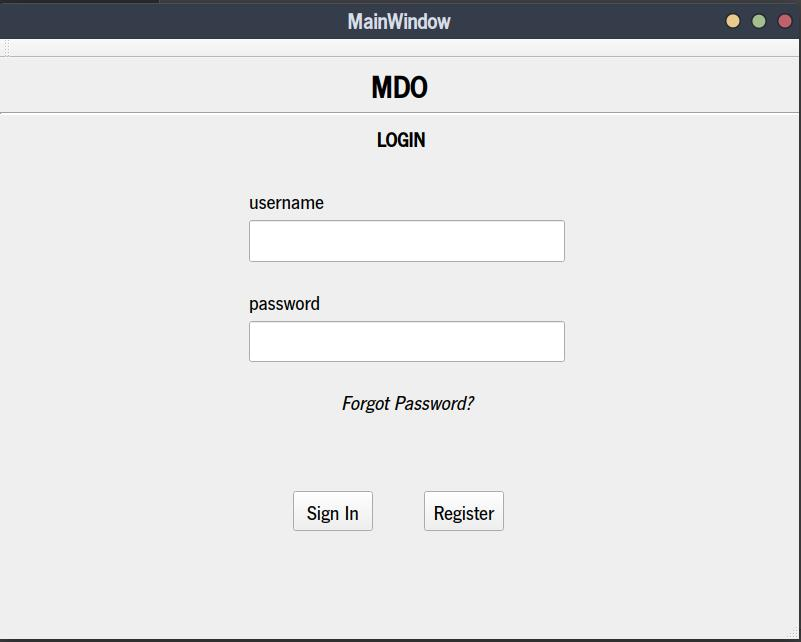
\includegraphics[width=\textwidth]{img/mw-login-view.jpg}%
  \caption{Login View}%
  \label{fig:mw-login-view}
\end{subfigure}

%\hspace{.1\textwidth}
%
  \begin{subfigure}{.6\textwidth}
    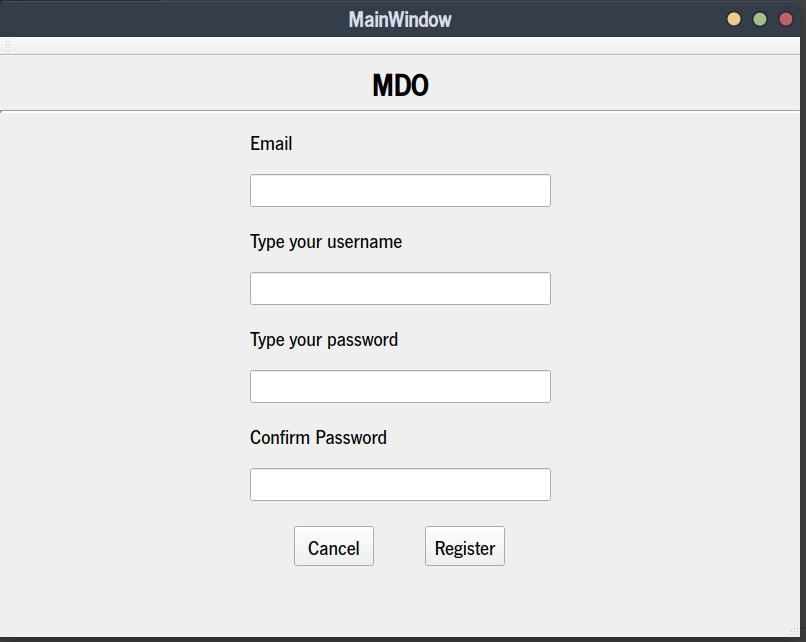
\includegraphics[width=\textwidth]{img/mw-register-view.jpg}%
  \caption{Register View}%
  \label{fig:mw-register-view}
  \end{subfigure}
  % 
  \caption{MainWindow views}%
  \label{fig:ptp-test}
\end{figure}  

\subsubsection{BrandWindow class}
%
The \texttt{BrandWindow} class is, as it suggests, the class that handles all of the brand's features.
This class handles all the transitions between views, such as \emph{Rent Ad View}, \emph{To Rent View} and \emph{Logout} - emits a signal to go back to login.
%
\lstinputlisting[language=c++, caption={Declaration of BrandWindow class},label=lst:brandwindow.h,
style=customc]{./listing/rc-brandwindow.h}%

As it can be seen in the header file of this class (listing \ref{lst:brandwindow.h}), there's also the session to handle the MySQL server connection (\texttt{Sess* sess}), a \texttt{QFileInfo} to handle the files to upload on an Ad and the \texttt{user\_id} which refers to the user that is currently using the app.
As in every part of the code, here there's also the usage of queues to the MySQL server, to rent ads and to see the ads rented to watch its statistics.
In order to make everything more simpler, in the \texttt{Rent View} it is only possible to rent for a range of one week. All the time slots that are already rented appear with a "Rented" \texttt{std::string} and the days that do not correspond to the time space available to rent appear with the label "Unavailable".

Perhaps, one of the most difficult functions to implement was the rent function, that's because it is necessary to add many rows to different tables in order to build a complete Ad on the database, this means that if something went wrong in the middle of the execution, it is necessary to do the inverse process to delete the already inserted rows, because they will not have a link to every tables.

Listing \ref{lst:rent-ad} shows the rent ad function.
%
\lstinputlisting[language=c++, firstline = 341, lastline=462, caption={Implementation of rent function on BrandWindow class},label=lst:rent-ad,
style=customc]{./listing/rc-brandwindow.cpp}

Because of the length and process capability of this function, every little mistake can take to serious consequences, so, it is mandatory to make all and every validation in order to avoid every mistake in the MySQL queue messages. Common errors can be such like redundant blocs of data, or even just a single piece of data.

\paragraph{\emph{Layout}}

Figures \ref{fig:brand-main-view}, \ref{fig:brand-to-rent-view} and \ref{fig:brand-rented-view} show the layout used for all the Brand Views.

\begin{figure}[htb!]
  \centering
  %
  \begin{subfigure}{.4\textwidth}
  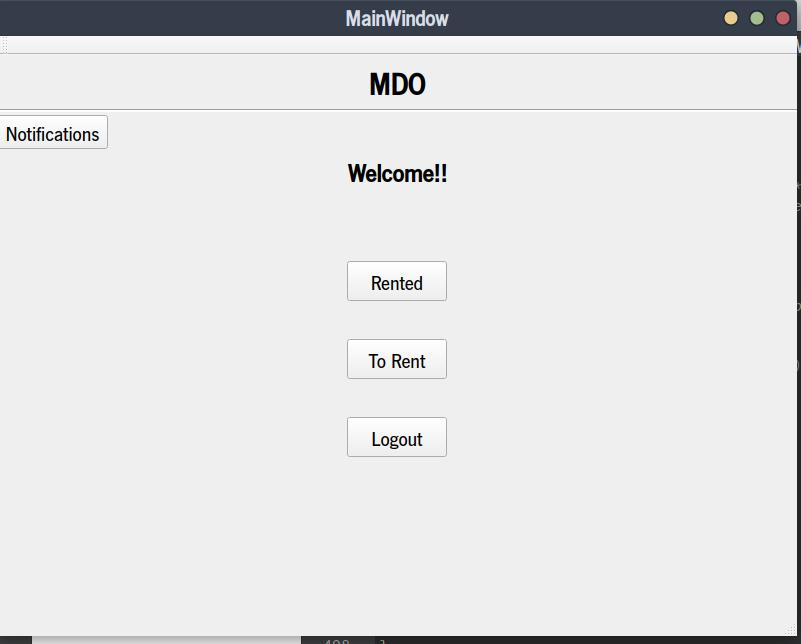
\includegraphics[width=\textwidth]{img/brand-main-view.jpg}%
  \caption{Brand Main View}%
  \label{fig:brand-main-view}
\end{subfigure}

%\hspace{.1\textwidth}
%
  \begin{subfigure}{.4\textwidth}
    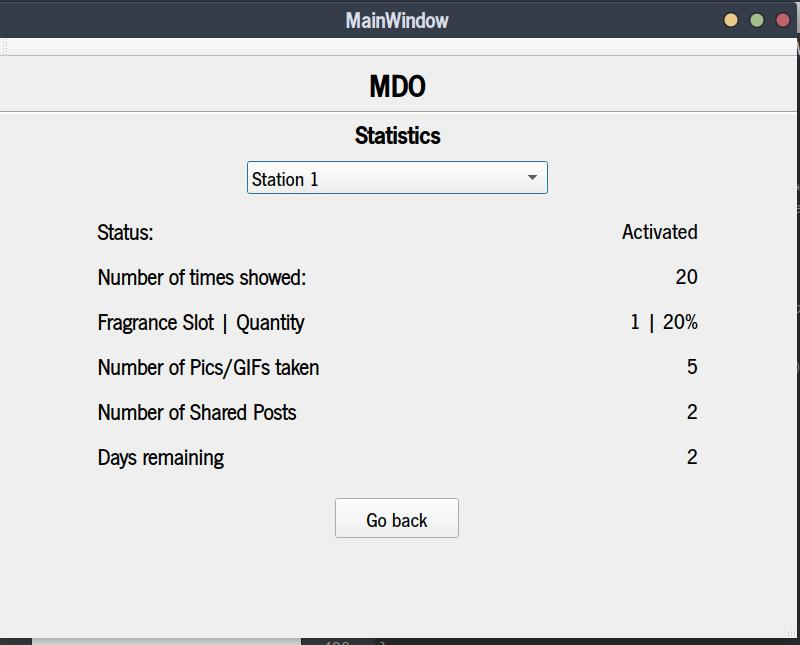
\includegraphics[width=\textwidth]{img/brand-rented-view.jpg}%
  \caption{Brand Rented View}%
  \label{fig:brand-rented-view}
  \end{subfigure}
  % 
  \begin{subfigure}{.4\textwidth}
    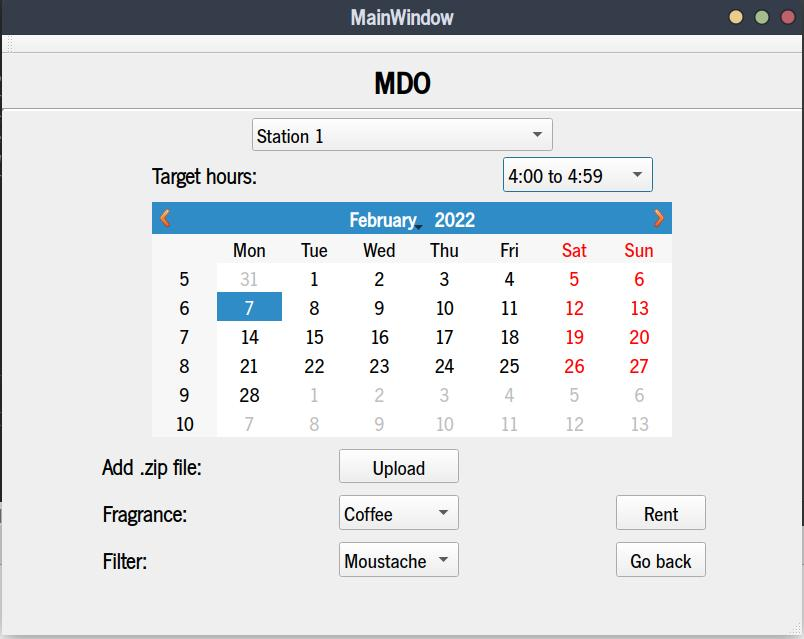
\includegraphics[width=\textwidth]{img/brand-to-rent-view.jpg}%
  \caption{Brand To Rent View}%
  \label{fig:brand-to-rent-view}
  \end{subfigure}
  % 
  \caption{BrandWindow views}%
  \label{fig:ptp-test}
\end{figure} 

\subsubsection{AdminWindow class}
%
The \texttt{AdmindWindow} class is, as it suggests, the class that handles all of the admin's features.
This class handles all the transitions between views, such as \emph{Statistics View}, \emph{Manage Users View}, \emph{Ads To Activate View} and \emph{Test Operation View}.
%
\lstinputlisting[language=c++, caption={Declaration of AdminWindow class},label=lst:adminwindow.h,
style=customc]{./listing/rc-adminwindow.h}%

In terms of private attributes, this class is similar to the \texttt{BrandWindow} class: it has a \texttt{Sess *sess} to handle the communication to MySQL server and it also has a \texttt{user\_id} to know which user is using the app.

Unfortunately, in this case it could not be implemented the Test Operation View because of reasons that will be explained in the next section.

As always, there's a lot of message queues to MySQL in order to handle all the data and shoe them in the \gls{mdo-rc}.
The most interesting feature in this class is the \textbf{Manage Users} function. In this view it is possible to change the permissions of a user, turning into an Admin or a Brand in just a click. It is also possible to delete users, which can be helpful to delete some bots or even users with bad conduct.
Also, the \textbf{Ads to Activate} is an interesting feature, because it can turn ads into active mode or, if denied, it can remove them. This feature is important once it is important to validate all data that is going to be sent to the machines, in order to avoid some type of non-advertisement videos that could appear in the stations.

Listing \ref{lst:admin-manage-users} shows the function \textbf{Manage Users}.
%
\lstinputlisting[language=c++, firstline=273, lastline=306, caption={Implementation of Manage Users from AdminWindow class},label=lst:admin-manage-users,
style=customc]{./listing/rc-adminwindow.cpp}%

Listing \ref{lst:admin-ads-to-act} shows the \textbf{Ads to Activate} feature.
%
\lstinputlisting[language=c++, firstline=376, lastline=430, caption={Implementation of Ads TO Activate from AdminWindow class},label=lst:admin-ads-to-act,
style=customc]{./listing/rc-adminwindow.cpp}%

\paragraph{\emph{Layout}}
%
On figures \ref{fig:admin-main-view}, \ref{fig:admin-manage-users-view} and \ref{fig:admin-ads-to-act-view} are all the views from the Admin Views.

\begin{figure}[htb!]
  \centering
  %
  \begin{subfigure}{.4\textwidth}
  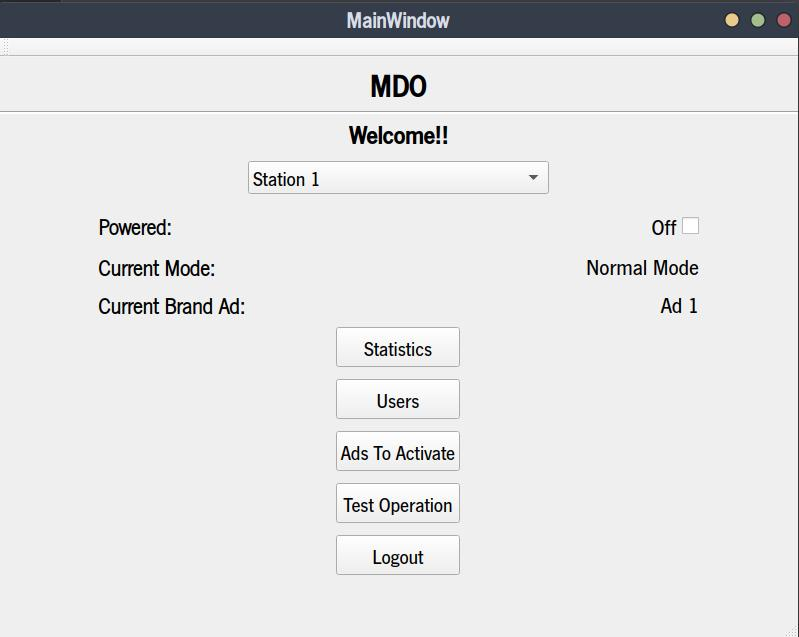
\includegraphics[width=\textwidth]{img/admin-main-view.jpg}%
  \caption{Admin Main View}%
  \label{fig:admin-main-view}
\end{subfigure}

%\hspace{.1\textwidth}
%
  \begin{subfigure}{.4\textwidth}
    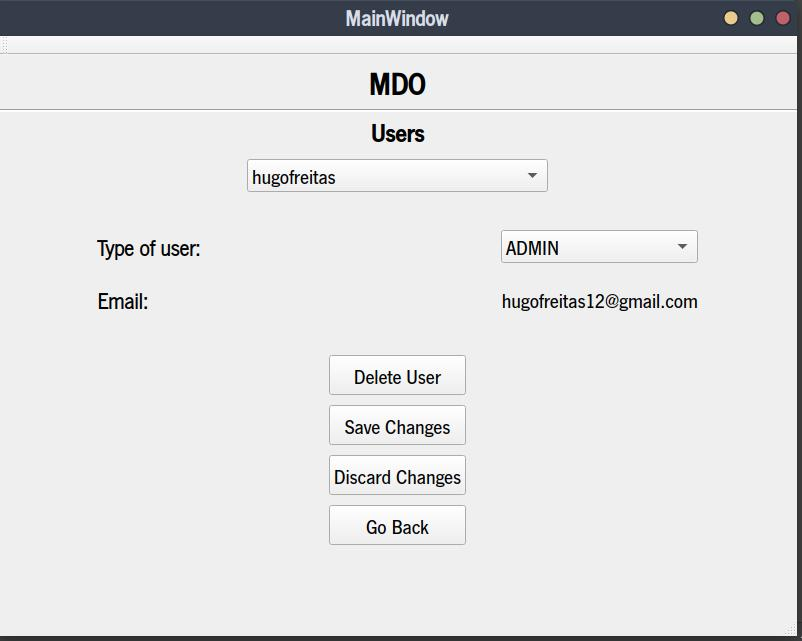
\includegraphics[width=\textwidth]{img/admin-manage-users-view.jpg}%
  \caption{Manage Users View}%
  \label{fig:admin-manage-users-view}
  \end{subfigure}
  % 
  \begin{subfigure}{.4\textwidth}
    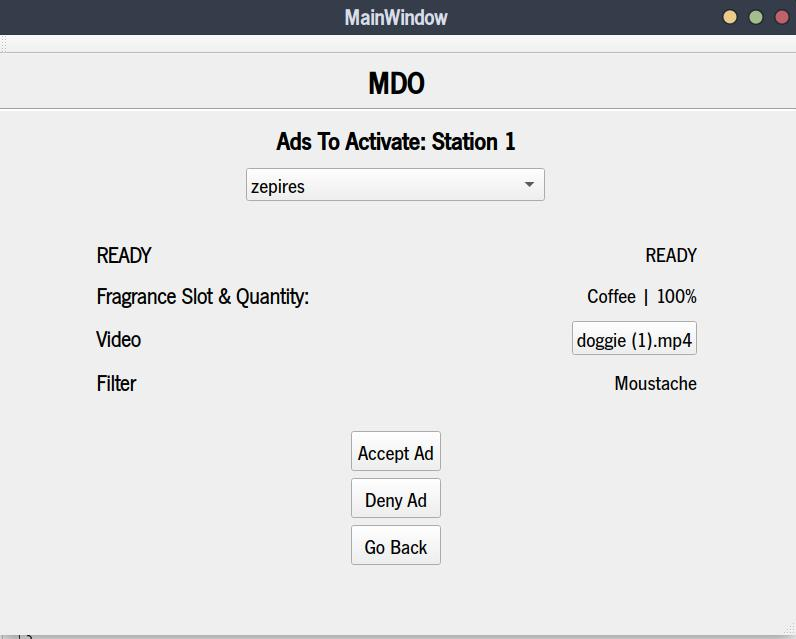
\includegraphics[width=\textwidth]{img/admin-ads-to-act.jpg}%
  \caption{Ads To Activate View}%
  \label{fig:admin-ads-to-act-view}
  \end{subfigure}
  % 
  \caption{AdminWindow views}%
  \label{fig:ptp-test}
\end{figure} 
\section{Remote Server}
\label{sec:rs}
%
The \gls{mdo-rs} was one of the subsystems previously designed to be implemented.
This application would give a more distributed architecture to the overall system.

Unfortunately, because of laps in time spent trying to resolve some unexpected issues and for many other variants, it turned out that it was not possible to develop a real Remote Server.
So, in terms to make everything work at its minimums, it was implemented a "kind of" Remote Server in the Remote Client.
This improvised Remote Server has a full database running in MySQL Server (as it could be seen before) and it has threads to create connections with clients - in this case, local systems - and send to them the information needed, such as new Ads information.

\subsection{Data Base}
The Data Base is one of the most important parts of this system for obvious reasons: this keeps all data stored and easy to access from the Remote Client and the Remote server.
Throughout its implementation, it suffered various iterations that were being stored in two different scripts, these scripts are \texttt{init.txt} (that initializes the Data Base) and \texttt{insert-values.txt} that populates the Data Base.
Implementing it by this way made everything more easy to develop because if it were errors on the Data Base, it was very fast to drop it, create it and populate it again.

Listing \ref{lst:init-sql} shows the init script to create the database.
%
\lstinputlisting[language=c++, caption={Script to create Data Base},label=lst:init-sql,
style=customc]{./listing/init.txt}%

Listing \ref{lst:populate-sql} shows the init script to create the database.
%
\lstinputlisting[language=c++, caption={Script to populate Data Base},label=lst:populate-sql,
style=customc]{./listing/init.txt}%

 

\subsection{Threads}
Looking back to Listing \ref{lst:mainwindow-h}, the threads that are being used are:
\begin{item-c}
\item \texttt{server\_thr} -- used to receive connections from other systems;
\item \texttt{receive\_from\_ls\_thr} -- used to receive messages from other systems;
\item \texttt{send\_to\_ls\_thr} -- used to send data to local system;
\item \texttt{update\_local\_system\_thr} -- updates the local system periodically.
\end{item-c}

\subsubsection{server\_thr}
In listing \ref{lst:server-thr} it is possible to take a look to the thread that waits for the connection of the local system.
%
\lstinputlisting[language=c++, firstline=413, lastline=463, caption={Implementation of Server Thread},label=lst:server-thr,
style=customc]{./listing/rc-mainwindow.cpp}%

This function creates a socket with a default port and starts the binding.
After a successes on binding, the thread blocks on \texttt{listen} to listen for an incoming connection.
As soon as it comes an incoming connection, the thread accepts it and runs the functions \texttt{connectionEneable} and stores the socket in order to keep the communication and signalize other functions that they can start sharing content with the local system.

\subsubsection{receive\_from\_ls\_thr}
In listing \ref{lst:recv-from-ls} is the implementation of the thread that receives messages from the local system.
%
\lstinputlisting[language=c++, firstline=492, lastline=505, caption={Implementation of Receive from \gls{mdo-l} Thread},label=lst:recv-from-ls,
style=customc]{./listing/rc-mainwindow.cpp}%

The function wait for the server to be connected to the local system, once that connection is established it blocks on the \texttt{recv}, waiting to receive something from the previously stored socket.

\subsubsection{send\_to\_ls\_thr}
Listing \ref{lst:send-to-ls} shows how the thread to send data to the local system works
%
\lstinputlisting[language=c++, firstline=507, lastline=530, caption={Implementation of Send to \gls{mdo-l} Thread},label=lst:send-to-ls,
style=customc]{./listing/rc-mainwindow.cpp}%

Firstly, as in the previous thread, it waits until connection is established. After that, it waits for a conditional signal that is sent when a timer expires. When that signal triggers to HIGH, it creates a frame to send that will be interpreted by the local system.

\subsubsection{update\_local\_system\_thr}
This function waits for a conditional signal to continue executing. This conditional signal is set when a timer expires, after that it jumps to the function \texttt{upload\_and\_update} that uploads the file with \texttt{curlpp} and then signalizes the previous function to execute.
%
\lstinputlisting[language=c++, firstline=264, lastline=288, caption={Implementation of Update \gls{mdo-l} Thread},label=lst:updt-ls,
style=customc]{./listing/rc-mainwindow.cpp}%

Obviously, this was the fastest way used to implement a Remote Server, encapsulating it in the Remote Client. In the future, all these threads will leave this app and will migrate and be adjusted to work in a more expandable and robust way.
\section{Local System}
\label{sec:test-ls}

The Local System is the most critical and more susceptible subsystem to cause errors. The probability of one error occur is bigger than on the other two subsystems and that's why this system is the one that needs to perform more test cases to be in the best performance possible.

The test cases can be divided in two main parts: hardware tests and software tests.

\subsection{Hardware Tests}
\label{subsec:ls-hw-tests}
%
There are many parts of hardware that need to be tested:
\begin{item-c}
\item Ultrasonic Sensors;
\item Fragrance Diffusion (Actuator and Module);
\item Camera;
\item Speakers;
\item Screen;
\end{item-c}

\subsubsection{Ultrasonic Sensors}
\label{sec:ussensors}

The ultrasonic sensors need to be with strong connections to all the supply sources and \gls{gpio} pins, after that, it has been ran a driver program that returned if the two sensors detected the presence of an obstacle. 
This program has a specific sample time that is more than enough to detect the presence of something in front of the sensors.
In fig.~\ref{fig:sensors-test} is the cable management of the sensors, while in fig.~\ref{fig:sensors-out-test} is the test output that ran as expected.
%
\begin{figure}[htb!]
  \centering
  \begin{subfigure}{.4\textwidth}
    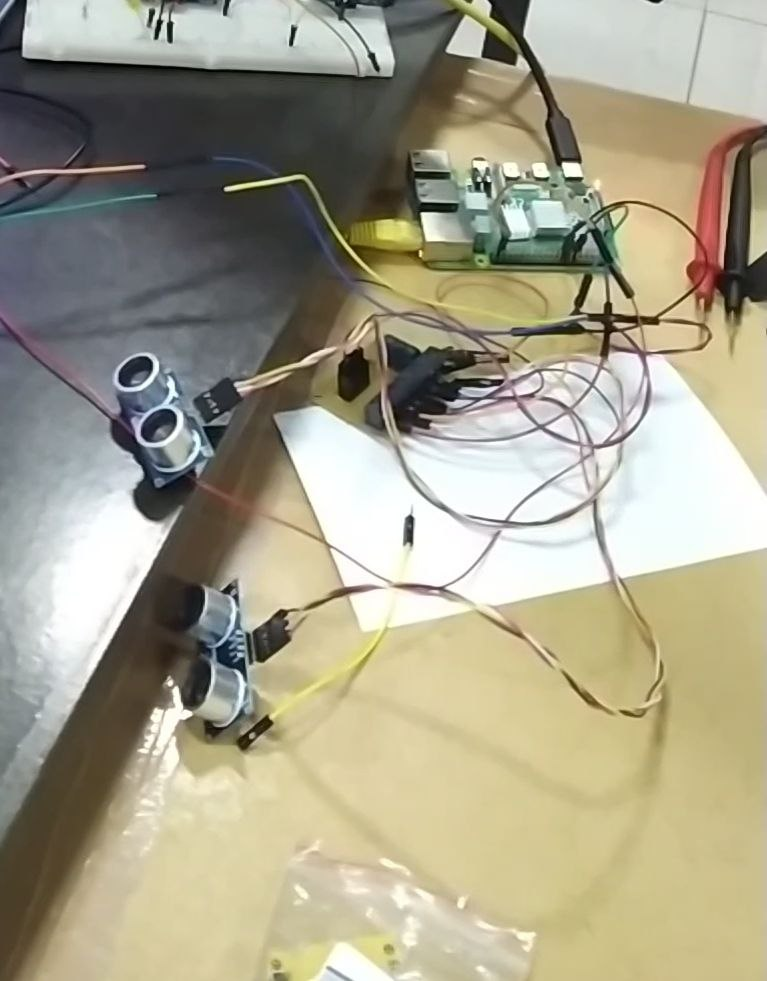
\includegraphics[width=\textwidth]{img/sensors-test.jpg}%
  \caption{Sensors Cable Management}%
  \label{fig:sensors-test}
  \end{subfigure}
  % 
  \begin{subfigure}{.5\textwidth}
    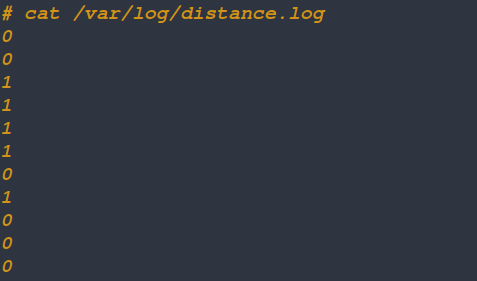
\includegraphics[width=\textwidth]{img/sensors-out-test.jpg}%
  \caption{Sensors Output Test}%
  \label{fig:sensors-out-test}
  \end{subfigure}
  % 
  \caption{Ultrasonic Sensors Test Cases}%
  \label{fig:uss-test}
\end{figure}

\subsubsection{Fragrance Diffusion (Actuator and Module)}
\label{sec:frag}

The fragrance diffuser module and its respective actuator need to be tested in order to respond to some signals gave by the main board.
In order for this to happen, it was tested with a driver program on the board and with all the module and it's components and the result was, as it can be seen in Fig.~\ref{fig:frag-test} what one expected.

\begin{figure}[!htb]
    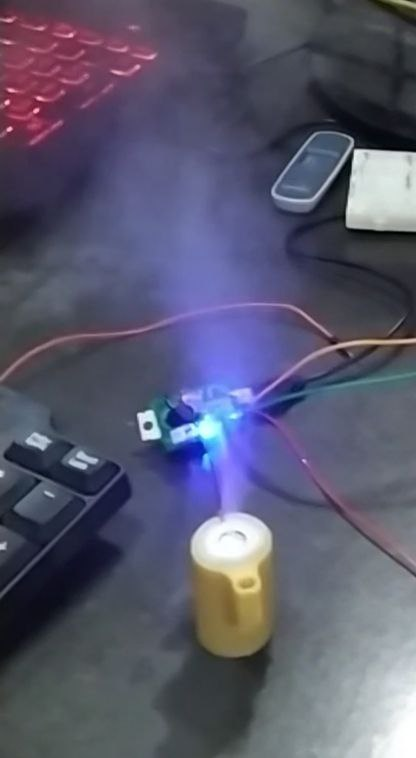
\includegraphics[width=.3\textwidth]{img/frag-test.jpg}%
  \caption{Fragrance Diffuser Output Test}%
  \label{fig:frag-test}
  \end{figure}
  
  
\subsubsection{Camera}
\label{sec:camera-test}
  
For the interaction mode it is mandatory that the camera module works properly to take pictures and gifs.
For this piece of hardware the test case is simple: turn on the camera and try to take a photo.

In this case it was used an image of Raspbian and with the help of an online app, the test of the camera worked as well as expected.
The result is on Fig.~\ref{fig:camera-test}.

\begin{figure}[!htb]
    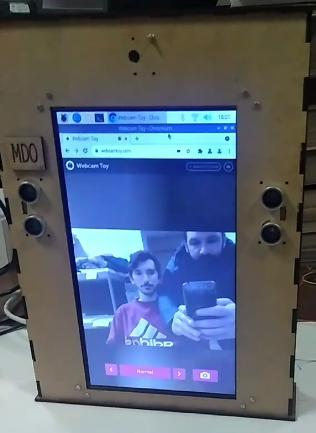
\includegraphics[width=.45\textwidth]{img/camera-teste.jpg}%
  \caption{Camera Output Test}%
  \label{fig:camera-test}
  \end{figure}
  
\subsubsection{Speakers}
\label{sec:speakers-test}

The speakers test cases are in a certain way different to test, because there's no way to show how it worked. However, the test was as simple as connect the speakers to the screen module board and play a video or an audio.

The audio played perfectly and the sound was well detected by human ears.

\subsubsection{Screen}
\label{sec:screen-test}

Testing the screen is similar to test the speakers. It's just simply connect the screen to the board and test its execution. As it can be seen in the previous figure when testing the camera (Fig.~\ref{sec:camera-test}) the screen was already being tested and it's more than proved that the screen works with no problems.


In conclusion, all hardware components and modules were tested successfully, which means that all test cases are now validated and it is possible to take the next step.


\section{Software}
\label{sec:software}
In this section the software tests conducted over the \texttt{Remote Client},
\texttt{Remote Server}, \texttt{Database} and \texttt{Local System} are presented.

\subsection{Local System}
\label{sec:local-system}
The \texttt{Local system} tests were performed on a host computer, prior to its
deployment to the \texttt{Raspberry Pi}. These tests are described next.

\subsubsection{Computer vision}
\label{sec:computer-vision-1}
In this section are described the frame acquisition,
face detection, and gesture recognition tests. Fig.~\ref{fig:cv-tests}
illustrates the combination of these tests. It can be seen that the camera
frames are acquired and processed to detect multiple faces and apply filters overlay, and
also to detect gestures that can be used to trigger UI events.
Additionally, it can be seen a picture that was taken, stored and displayed,
which is ready for sharing on social media.
\begin{figure}[htb!]
\centering
    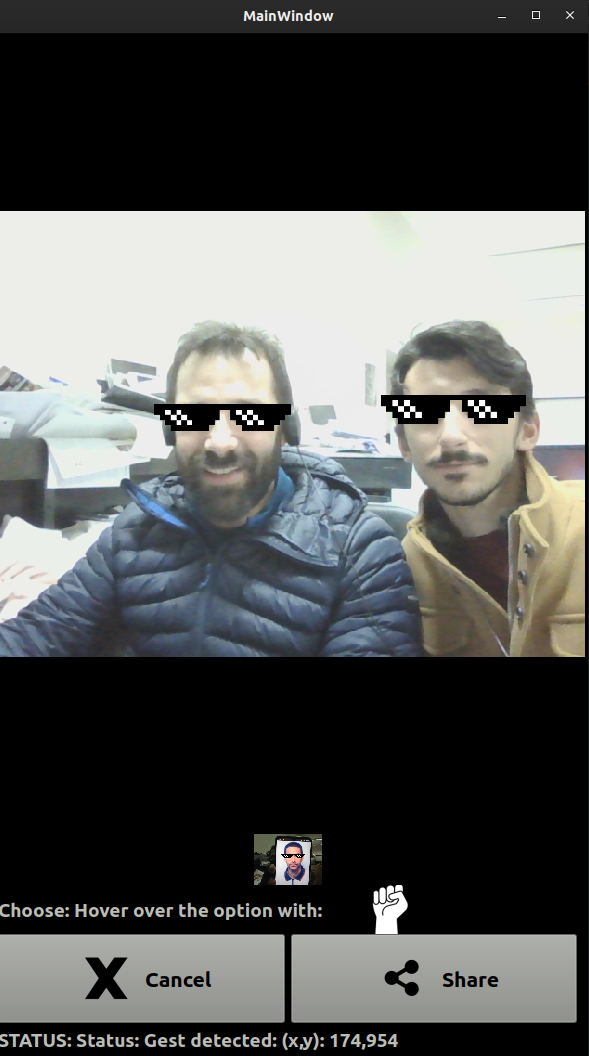
\includegraphics[width=0.6\textwidth]{./img/UI-test-filters.png}
  \caption{Computer visions tests}%
\label{fig:cv-tests}
\end{figure}

\subsubsection{Normal mode}
\label{sec:normal-mode}
Fig.~\ref{fig:normal-mode-test} illustrates the normal mode testing. It
demonstrated that a video can be reproduced on a loop while the fragrance
diffuser was also enabled and disabled according to its on and off times. The
normal mode only exited if there was no current ad enabled or if a user was
detected.
%
\begin{figure}[htb!]
\centering
    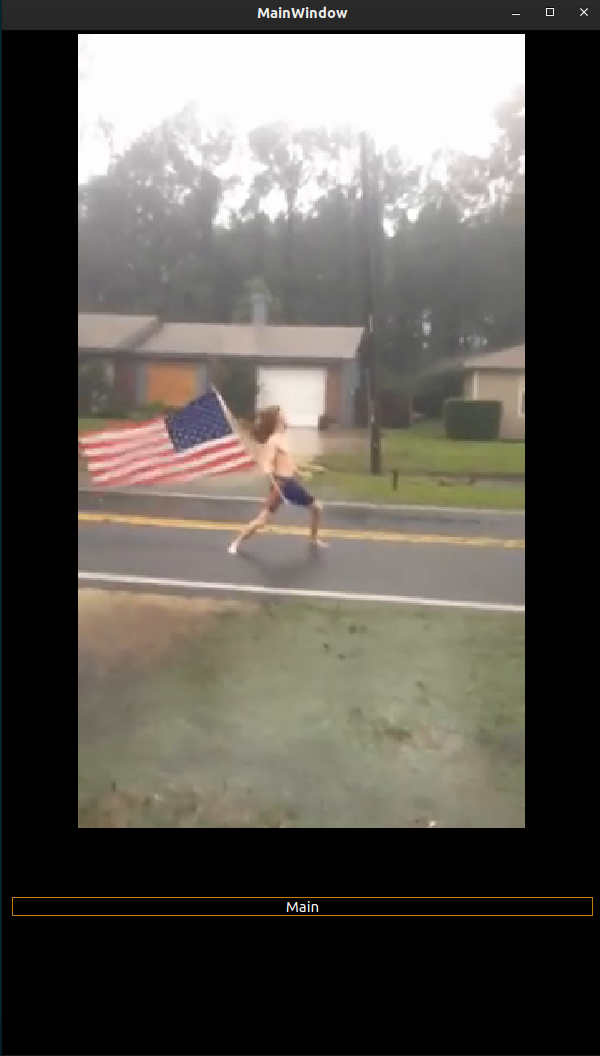
\includegraphics[width=0.6\textwidth]{./img/ui-test-normal-mode.png}
  \caption{Normal mode: testing}%
\label{fig:normal-mode-test}
\end{figure}

\subsubsection{Interaction mode}
\label{sec:interaction-mode}
The interaction mode tests demonstrated that it was possible to take pictures
and create GIFs on demand, as illustrated in Fig.~\ref{fig:cv-tests}.

\subsubsection{Twitter sharing}
\label{sec:twitter-sharing}
Fig.~\ref{fig:twitter-test} illustrates the Twitter sharing mode. It
demonstrated that a post can be successfully shared from the Local System into
Twitter. Nonetheless, at the current time, it is still not possible to upload
media to Twitter, as the API recently changed, requiring extra time to implement.
%
\begin{figure}[htb!]
  \centering
  % 
  \begin{subfigure}[t]{.4\textwidth}
  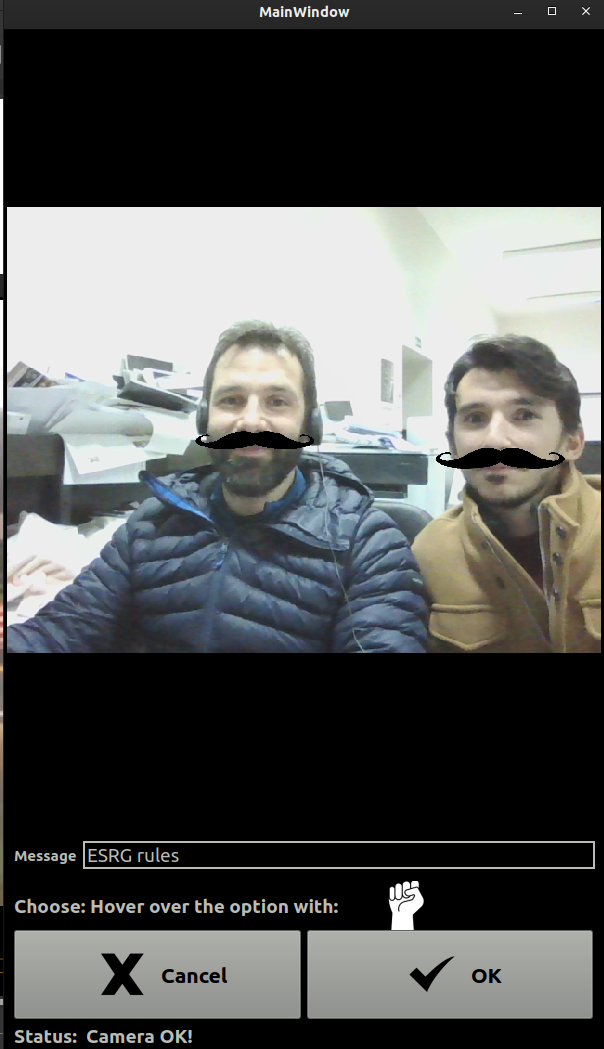
\includegraphics[width=\textwidth]{img/ui-test-sharing-mode.png}%
  %\caption{main}%
  %\label{fig:state-mach-local-superv-main}
\end{subfigure}
%
\hspace{.05\textwidth}
%
  \begin{subfigure}[t]{.42\textwidth}
  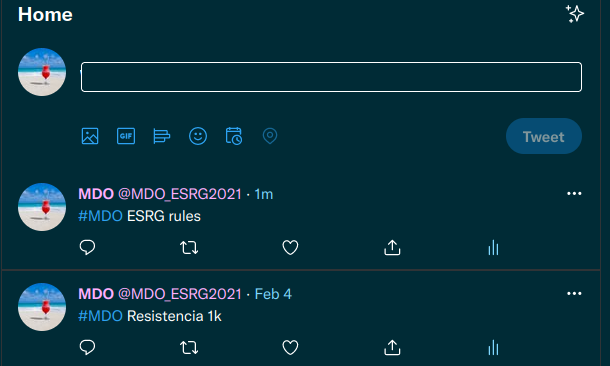
\includegraphics[width=\textwidth]{img/ui-test-sharing-mode2.png}%
  %\caption{Request Handler}%
  %\label{fig:state-mach-local-superv-req}
\end{subfigure}
  % 
  \caption{Twitter sharing: testing}%
  \label{fig:twitter-test}
\end{figure}
%

\subsubsection{Image filtering mode}
\label{sec:image-filtering-mode}
From Fig.~\ref{fig:cv-tests} and Fig.~\ref{fig:twitter-test}, it is possible to
verify that several filters were successfully implemented. Moreover, it is
possible to observe from the last figure that the image filter can be persistent
if desired.

\subsubsection{Download Ad}
\label{sec:download-ad}
Fig.~\ref{fig:download-test} illustrates the download of an Ad in the
background, while the application was currently busy in the interaction mode.
%
\begin{figure}[htb!]
\centering
    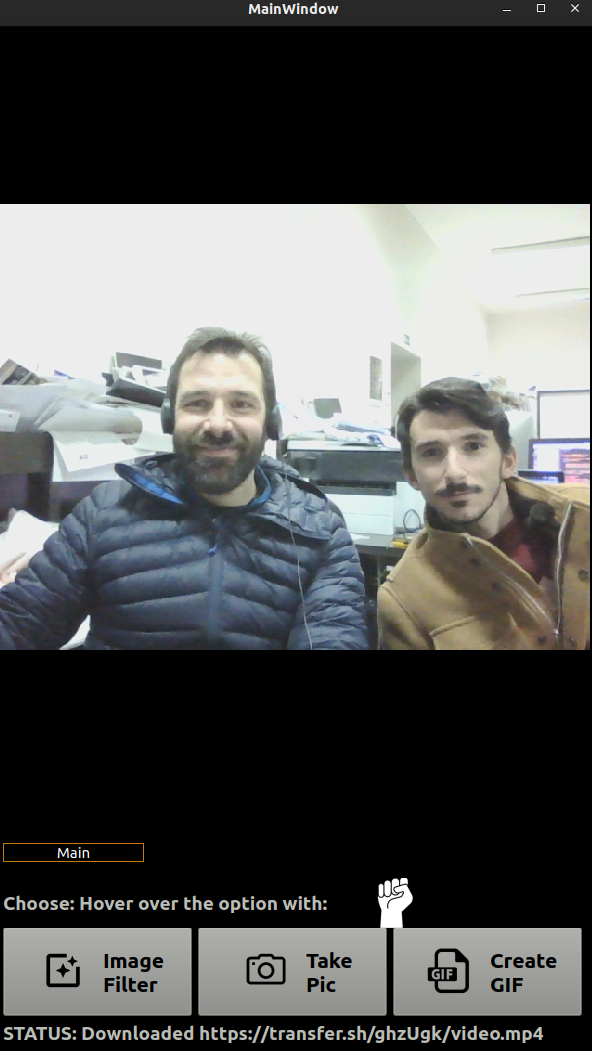
\includegraphics[width=0.6\textwidth]{./img/ui-test-download-ad.png}
  \caption{Download Ad: testing}%
\label{fig:download-test}
\end{figure}


\subsubsection{Connection to Remote System}
\label{sec:conn-remote-syst}
The connection to the remote system was simulated and tested deploying a server
listening in the \texttt{localhost} and observing the connection and data exchange between the two
nodes. This test was successful validating the client-server architecture logic
and implementation.

\subsubsection{User detection}
\label{sec:user-detection}
The user detection was tested by deploying the user detection daemon to
stimulate the application. It was verified that the daemon successfully detects
the ultrasonic sensors triggering when a person passes and that this event is
conveyed to the local system via message queue where it is successfully
detected, signaling a user was detected.

%%% Local Variables:
%%% mode: latex
%%% TeX-master: "../../../dissertation"
%%% End:
